
\begin{frame}
  \frametitle{Paparazzi: A UAV System}

  \begin{center}
    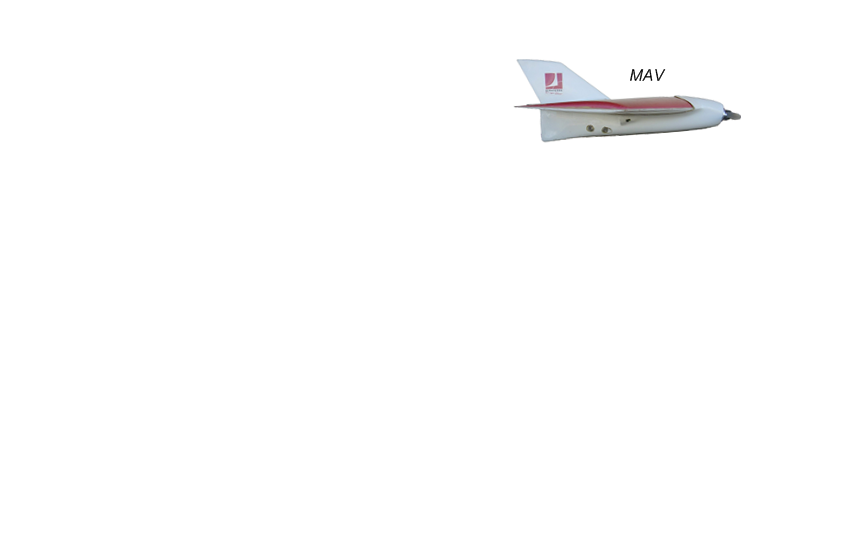
\includegraphics[height=6cm]{system/system_overview_0}<1>
    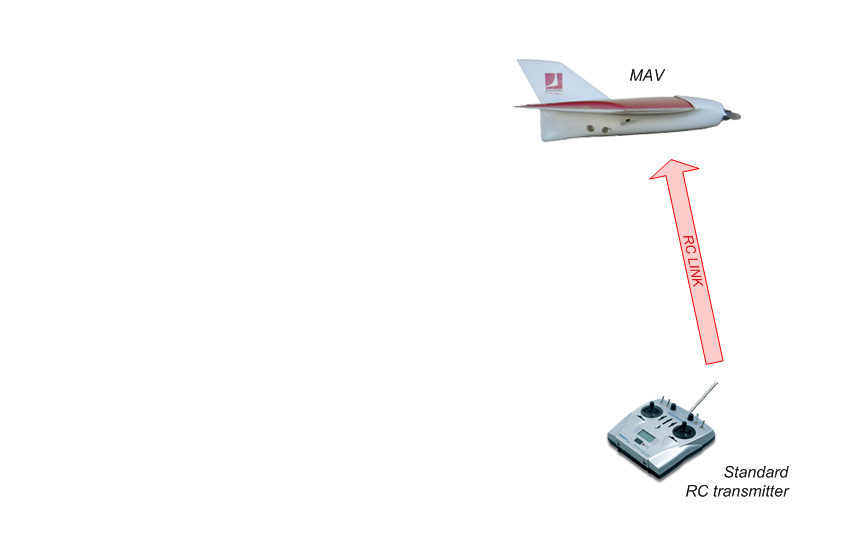
\includegraphics[height=6cm]{system/system_overview_1}<2>
    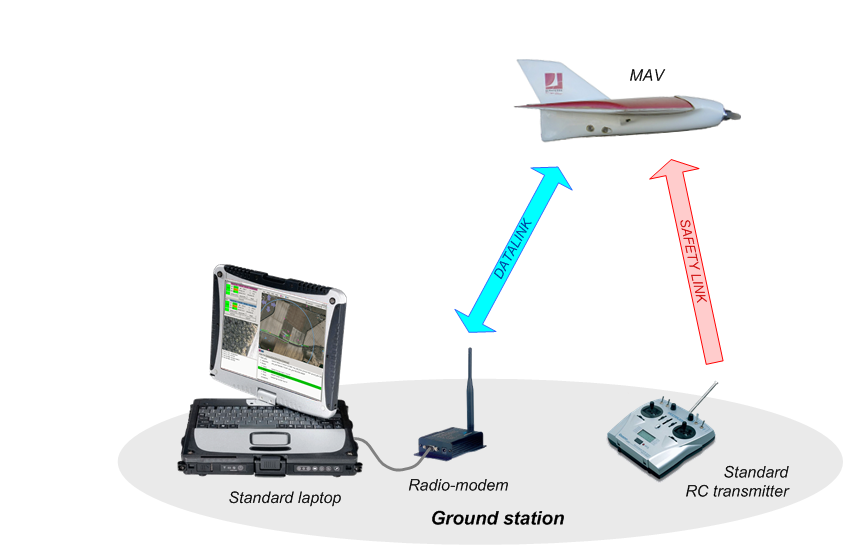
\includegraphics[height=6cm]{system/system_overview_2}<3>
    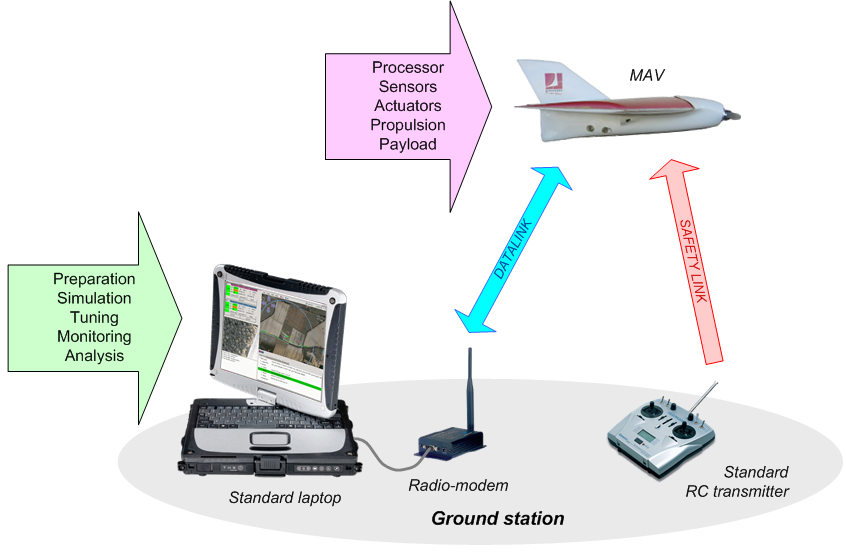
\includegraphics[height=6cm]{system/system_overview_3}<4>
  \end{center}
\end{frame}

%
% Features
%
\subsection{Features}

% control
% - augmented stability
% - waypoint navitation
% - complex trajectories
% - dynamic trajectories ( search patterns )


%
% Networked architecture
\begin{frame}
\frametitle{Architecture}
\begin{center}
Multi-aircraft network enabled ground segment
\end{center}
\begin{center}
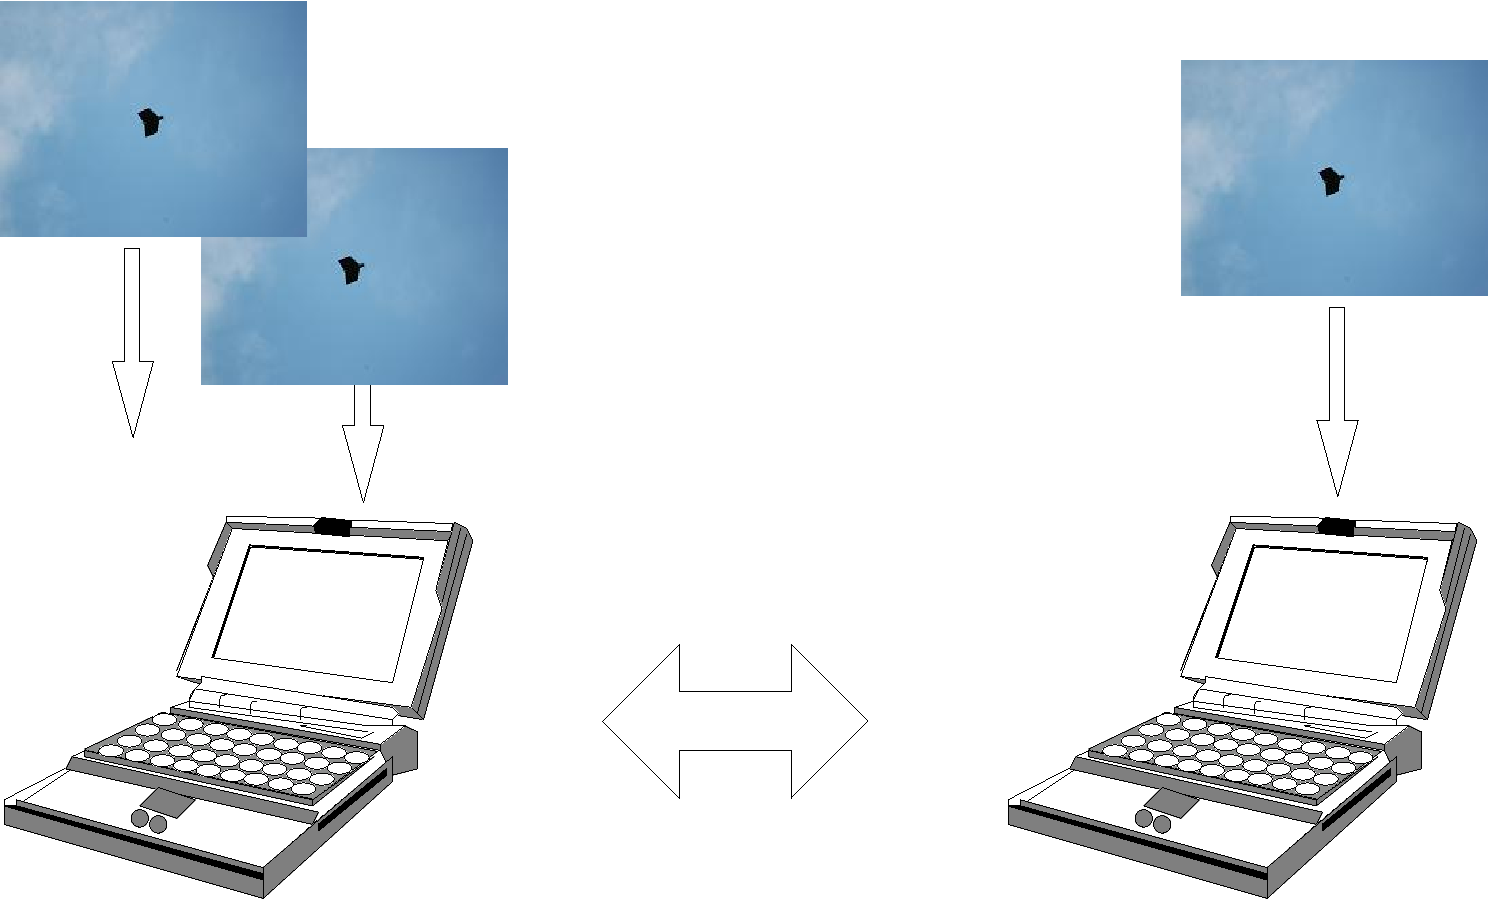
\includegraphics[height=4cm]{system/network}
\end{center}
\end{frame}


% configuration
% simulation
% flight
% analysis
% replay


%
% Ground station
\begin{frame}
  \frametitle{Multi-UAV Human Machine Interface}

  \begin{center}
    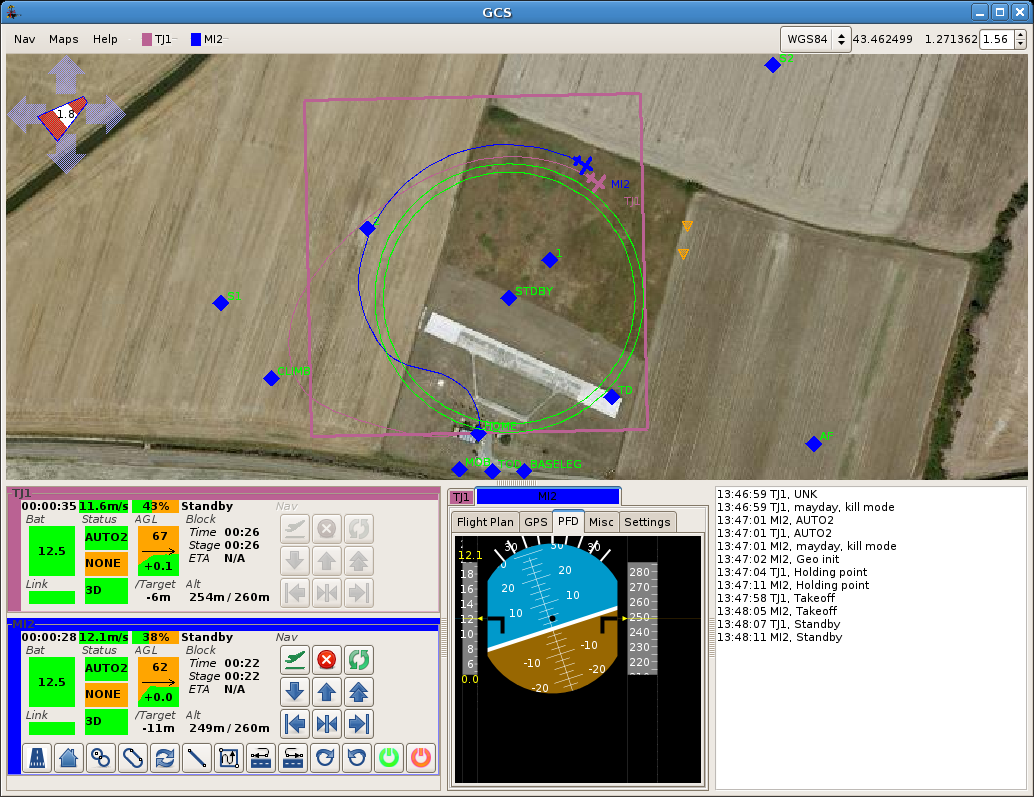
\includegraphics[height=7cm]{gcs/overall}
  \end{center}
\end{frame}


%
% Control board
\begin{frame}
  \frametitle{Controller board}
  \begin{center}
    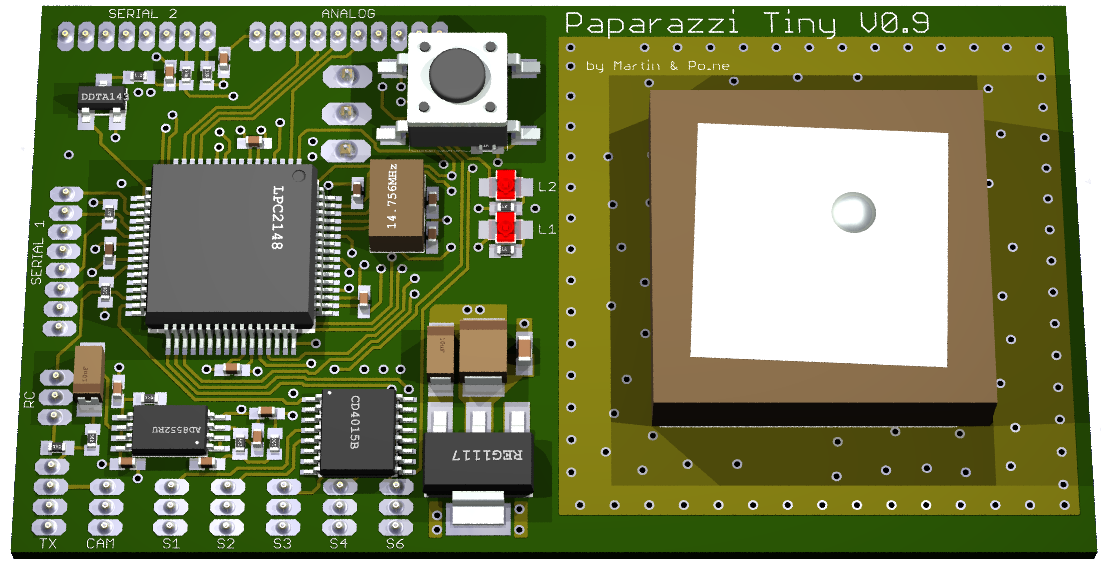
\includegraphics[width=7cm]{control_board/tiny_cad_top.png}
   
    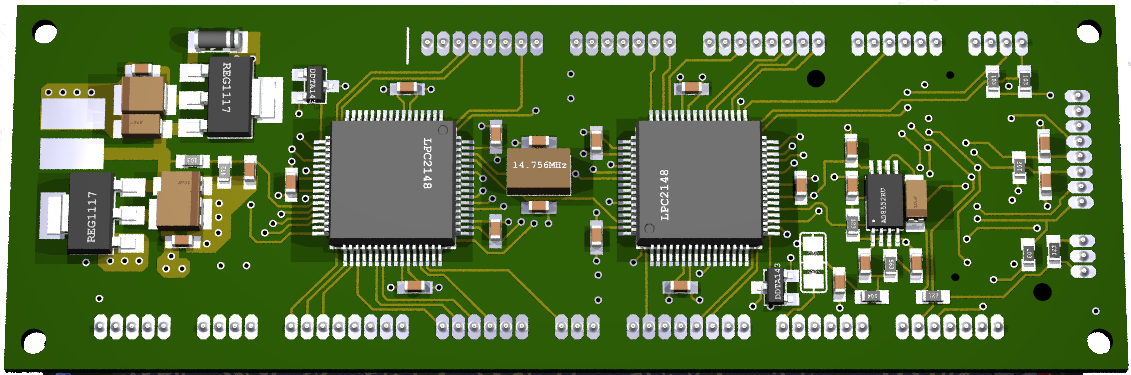
\includegraphics[width=8cm]{control_board/classix_cad_top.png}    
  \end{center}
\end{frame}


%
% Sensors



%
% Video
\begin{frame}
\frametitle{Video}

\begin{columns}
\begin{column}{5cm}
\begin{itemize}
\item Real-time video downlink
\item Footprint on map
\item Network streaming
\item Stitching
\item Smoke detection
\end{itemize}
\end{column}
\begin{column}{5cm}
\begin{center}
\movie[externalviewer=gxine]{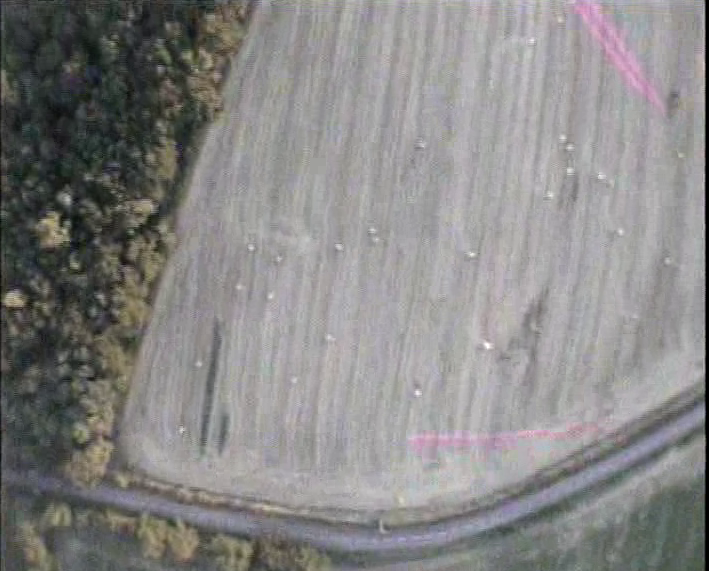
\includegraphics[height=3cm]{aerial/montfaucon}}{../video/montfaucon.avi}
\end{center}
\end{column}
\end{columns}
\begin{center}
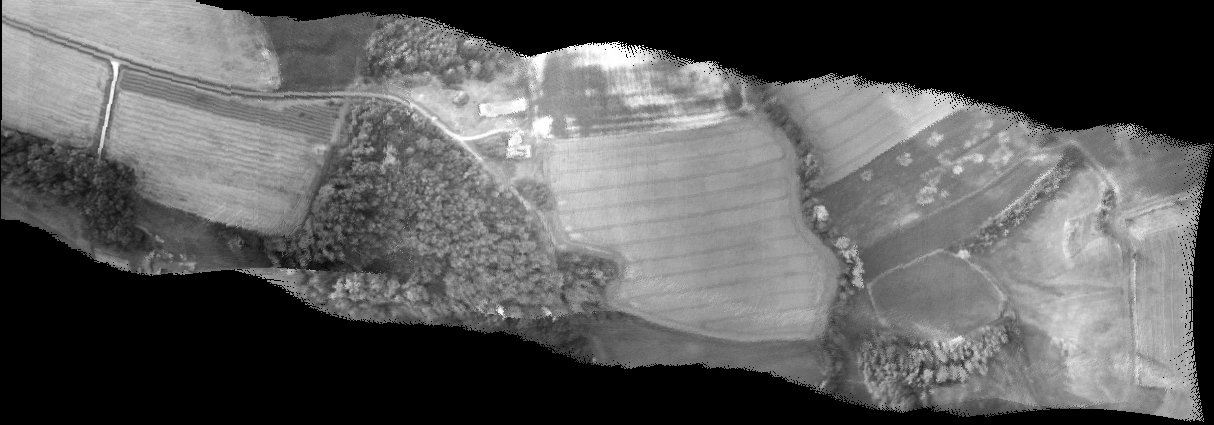
\includegraphics[width=9cm]{aerial/collage_adrien}<1>
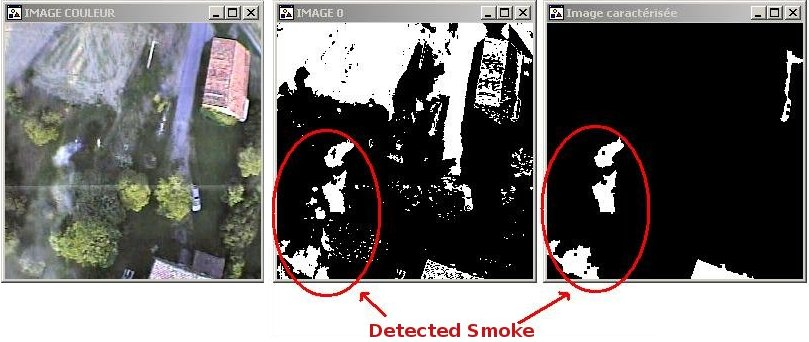
\includegraphics[width=9cm]{aerial/video8}<2>
\end{center}
\end{frame}


%
% History
%
\subsection{History}
